\documentclass{article}
\usepackage{iclr2027_conference,times}
%%%%% NEW MATH DEFINITIONS %%%%%

\usepackage{amsmath,amsfonts,bm}

% Mark sections of captions for referring to divisions of figures
\newcommand{\figleft}{{\em (Left)}}
\newcommand{\figcenter}{{\em (Center)}}
\newcommand{\figright}{{\em (Right)}}
\newcommand{\figtop}{{\em (Top)}}
\newcommand{\figbottom}{{\em (Bottom)}}
\newcommand{\captiona}{{\em (a)}}
\newcommand{\captionb}{{\em (b)}}
\newcommand{\captionc}{{\em (c)}}
\newcommand{\captiond}{{\em (d)}}

% Highlight a newly defined term
\newcommand{\newterm}[1]{{\bf #1}}


% Figure reference, lower-case.
\def\figref#1{figure~\ref{#1}}
% Figure reference, capital. For start of sentence
\def\Figref#1{Figure~\ref{#1}}
\def\twofigref#1#2{figures \ref{#1} and \ref{#2}}
\def\quadfigref#1#2#3#4{figures \ref{#1}, \ref{#2}, \ref{#3} and \ref{#4}}
% Section reference, lower-case.
\def\secref#1{section~\ref{#1}}
% Section reference, capital.
\def\Secref#1{Section~\ref{#1}}
% Reference to two sections.
\def\twosecrefs#1#2{sections \ref{#1} and \ref{#2}}
% Reference to three sections.
\def\secrefs#1#2#3{sections \ref{#1}, \ref{#2} and \ref{#3}}
% Reference to an equation, lower-case.
\def\eqref#1{equation~\ref{#1}}
% Reference to an equation, upper case
\def\Eqref#1{Equation~\ref{#1}}
% A raw reference to an equation---avoid using if possible
\def\plaineqref#1{\ref{#1}}
% Reference to a chapter, lower-case.
\def\chapref#1{chapter~\ref{#1}}
% Reference to an equation, upper case.
\def\Chapref#1{Chapter~\ref{#1}}
% Reference to a range of chapters
\def\rangechapref#1#2{chapters\ref{#1}--\ref{#2}}
% Reference to an algorithm, lower-case.
\def\algref#1{algorithm~\ref{#1}}
% Reference to an algorithm, upper case.
\def\Algref#1{Algorithm~\ref{#1}}
\def\twoalgref#1#2{algorithms \ref{#1} and \ref{#2}}
\def\Twoalgref#1#2{Algorithms \ref{#1} and \ref{#2}}
% Reference to a part, lower case
\def\partref#1{part~\ref{#1}}
% Reference to a part, upper case
\def\Partref#1{Part~\ref{#1}}
\def\twopartref#1#2{parts \ref{#1} and \ref{#2}}

\def\ceil#1{\lceil #1 \rceil}
\def\floor#1{\lfloor #1 \rfloor}
\def\1{\bm{1}}
\newcommand{\train}{\mathcal{D}}
\newcommand{\valid}{\mathcal{D_{\mathrm{valid}}}}
\newcommand{\test}{\mathcal{D_{\mathrm{test}}}}

\def\eps{{\epsilon}}


% Random variables
\def\reta{{\textnormal{$\eta$}}}
\def\ra{{\textnormal{a}}}
\def\rb{{\textnormal{b}}}
\def\rc{{\textnormal{c}}}
\def\rd{{\textnormal{d}}}
\def\re{{\textnormal{e}}}
\def\rf{{\textnormal{f}}}
\def\rg{{\textnormal{g}}}
\def\rh{{\textnormal{h}}}
\def\ri{{\textnormal{i}}}
\def\rj{{\textnormal{j}}}
\def\rk{{\textnormal{k}}}
\def\rl{{\textnormal{l}}}
% rm is already a command, just don't name any random variables m
\def\rn{{\textnormal{n}}}
\def\ro{{\textnormal{o}}}
\def\rp{{\textnormal{p}}}
\def\rq{{\textnormal{q}}}
\def\rr{{\textnormal{r}}}
\def\rs{{\textnormal{s}}}
\def\rt{{\textnormal{t}}}
\def\ru{{\textnormal{u}}}
\def\rv{{\textnormal{v}}}
\def\rw{{\textnormal{w}}}
\def\rx{{\textnormal{x}}}
\def\ry{{\textnormal{y}}}
\def\rz{{\textnormal{z}}}

% Random vectors
\def\rvepsilon{{\mathbf{\epsilon}}}
\def\rvtheta{{\mathbf{\theta}}}
\def\rva{{\mathbf{a}}}
\def\rvb{{\mathbf{b}}}
\def\rvc{{\mathbf{c}}}
\def\rvd{{\mathbf{d}}}
\def\rve{{\mathbf{e}}}
\def\rvf{{\mathbf{f}}}
\def\rvg{{\mathbf{g}}}
\def\rvh{{\mathbf{h}}}
\def\rvu{{\mathbf{i}}}
\def\rvj{{\mathbf{j}}}
\def\rvk{{\mathbf{k}}}
\def\rvl{{\mathbf{l}}}
\def\rvm{{\mathbf{m}}}
\def\rvn{{\mathbf{n}}}
\def\rvo{{\mathbf{o}}}
\def\rvp{{\mathbf{p}}}
\def\rvq{{\mathbf{q}}}
\def\rvr{{\mathbf{r}}}
\def\rvs{{\mathbf{s}}}
\def\rvt{{\mathbf{t}}}
\def\rvu{{\mathbf{u}}}
\def\rvv{{\mathbf{v}}}
\def\rvw{{\mathbf{w}}}
\def\rvx{{\mathbf{x}}}
\def\rvy{{\mathbf{y}}}
\def\rvz{{\mathbf{z}}}

% Elements of random vectors
\def\erva{{\textnormal{a}}}
\def\ervb{{\textnormal{b}}}
\def\ervc{{\textnormal{c}}}
\def\ervd{{\textnormal{d}}}
\def\erve{{\textnormal{e}}}
\def\ervf{{\textnormal{f}}}
\def\ervg{{\textnormal{g}}}
\def\ervh{{\textnormal{h}}}
\def\ervi{{\textnormal{i}}}
\def\ervj{{\textnormal{j}}}
\def\ervk{{\textnormal{k}}}
\def\ervl{{\textnormal{l}}}
\def\ervm{{\textnormal{m}}}
\def\ervn{{\textnormal{n}}}
\def\ervo{{\textnormal{o}}}
\def\ervp{{\textnormal{p}}}
\def\ervq{{\textnormal{q}}}
\def\ervr{{\textnormal{r}}}
\def\ervs{{\textnormal{s}}}
\def\ervt{{\textnormal{t}}}
\def\ervu{{\textnormal{u}}}
\def\ervv{{\textnormal{v}}}
\def\ervw{{\textnormal{w}}}
\def\ervx{{\textnormal{x}}}
\def\ervy{{\textnormal{y}}}
\def\ervz{{\textnormal{z}}}

% Random matrices
\def\rmA{{\mathbf{A}}}
\def\rmB{{\mathbf{B}}}
\def\rmC{{\mathbf{C}}}
\def\rmD{{\mathbf{D}}}
\def\rmE{{\mathbf{E}}}
\def\rmF{{\mathbf{F}}}
\def\rmG{{\mathbf{G}}}
\def\rmH{{\mathbf{H}}}
\def\rmI{{\mathbf{I}}}
\def\rmJ{{\mathbf{J}}}
\def\rmK{{\mathbf{K}}}
\def\rmL{{\mathbf{L}}}
\def\rmM{{\mathbf{M}}}
\def\rmN{{\mathbf{N}}}
\def\rmO{{\mathbf{O}}}
\def\rmP{{\mathbf{P}}}
\def\rmQ{{\mathbf{Q}}}
\def\rmR{{\mathbf{R}}}
\def\rmS{{\mathbf{S}}}
\def\rmT{{\mathbf{T}}}
\def\rmU{{\mathbf{U}}}
\def\rmV{{\mathbf{V}}}
\def\rmW{{\mathbf{W}}}
\def\rmX{{\mathbf{X}}}
\def\rmY{{\mathbf{Y}}}
\def\rmZ{{\mathbf{Z}}}

% Elements of random matrices
\def\ermA{{\textnormal{A}}}
\def\ermB{{\textnormal{B}}}
\def\ermC{{\textnormal{C}}}
\def\ermD{{\textnormal{D}}}
\def\ermE{{\textnormal{E}}}
\def\ermF{{\textnormal{F}}}
\def\ermG{{\textnormal{G}}}
\def\ermH{{\textnormal{H}}}
\def\ermI{{\textnormal{I}}}
\def\ermJ{{\textnormal{J}}}
\def\ermK{{\textnormal{K}}}
\def\ermL{{\textnormal{L}}}
\def\ermM{{\textnormal{M}}}
\def\ermN{{\textnormal{N}}}
\def\ermO{{\textnormal{O}}}
\def\ermP{{\textnormal{P}}}
\def\ermQ{{\textnormal{Q}}}
\def\ermR{{\textnormal{R}}}
\def\ermS{{\textnormal{S}}}
\def\ermT{{\textnormal{T}}}
\def\ermU{{\textnormal{U}}}
\def\ermV{{\textnormal{V}}}
\def\ermW{{\textnormal{W}}}
\def\ermX{{\textnormal{X}}}
\def\ermY{{\textnormal{Y}}}
\def\ermZ{{\textnormal{Z}}}

% Vectors
\def\vzero{{\bm{0}}}
\def\vone{{\bm{1}}}
\def\vmu{{\bm{\mu}}}
\def\vtheta{{\bm{\theta}}}
\def\va{{\bm{a}}}
\def\vb{{\bm{b}}}
\def\vc{{\bm{c}}}
\def\vd{{\bm{d}}}
\def\ve{{\bm{e}}}
\def\vf{{\bm{f}}}
\def\vg{{\bm{g}}}
\def\vh{{\bm{h}}}
\def\vi{{\bm{i}}}
\def\vj{{\bm{j}}}
\def\vk{{\bm{k}}}
\def\vl{{\bm{l}}}
\def\vm{{\bm{m}}}
\def\vn{{\bm{n}}}
\def\vo{{\bm{o}}}
\def\vp{{\bm{p}}}
\def\vq{{\bm{q}}}
\def\vr{{\bm{r}}}
\def\vs{{\bm{s}}}
\def\vt{{\bm{t}}}
\def\vu{{\bm{u}}}
\def\vv{{\bm{v}}}
\def\vw{{\bm{w}}}
\def\vx{{\bm{x}}}
\def\vy{{\bm{y}}}
\def\vz{{\bm{z}}}

% Elements of vectors
\def\evalpha{{\alpha}}
\def\evbeta{{\beta}}
\def\evepsilon{{\epsilon}}
\def\evlambda{{\lambda}}
\def\evomega{{\omega}}
\def\evmu{{\mu}}
\def\evpsi{{\psi}}
\def\evsigma{{\sigma}}
\def\evtheta{{\theta}}
\def\eva{{a}}
\def\evb{{b}}
\def\evc{{c}}
\def\evd{{d}}
\def\eve{{e}}
\def\evf{{f}}
\def\evg{{g}}
\def\evh{{h}}
\def\evi{{i}}
\def\evj{{j}}
\def\evk{{k}}
\def\evl{{l}}
\def\evm{{m}}
\def\evn{{n}}
\def\evo{{o}}
\def\evp{{p}}
\def\evq{{q}}
\def\evr{{r}}
\def\evs{{s}}
\def\evt{{t}}
\def\evu{{u}}
\def\evv{{v}}
\def\evw{{w}}
\def\evx{{x}}
\def\evy{{y}}
\def\evz{{z}}

% Matrix
\def\mA{{\bm{A}}}
\def\mB{{\bm{B}}}
\def\mC{{\bm{C}}}
\def\mD{{\bm{D}}}
\def\mE{{\bm{E}}}
\def\mF{{\bm{F}}}
\def\mG{{\bm{G}}}
\def\mH{{\bm{H}}}
\def\mI{{\bm{I}}}
\def\mJ{{\bm{J}}}
\def\mK{{\bm{K}}}
\def\mL{{\bm{L}}}
\def\mM{{\bm{M}}}
\def\mN{{\bm{N}}}
\def\mO{{\bm{O}}}
\def\mP{{\bm{P}}}
\def\mQ{{\bm{Q}}}
\def\mR{{\bm{R}}}
\def\mS{{\bm{S}}}
\def\mT{{\bm{T}}}
\def\mU{{\bm{U}}}
\def\mV{{\bm{V}}}
\def\mW{{\bm{W}}}
\def\mX{{\bm{X}}}
\def\mY{{\bm{Y}}}
\def\mZ{{\bm{Z}}}
\def\mBeta{{\bm{\beta}}}
\def\mPhi{{\bm{\Phi}}}
\def\mLambda{{\bm{\Lambda}}}
\def\mSigma{{\bm{\Sigma}}}

% Tensor
\DeclareMathAlphabet{\mathsfit}{\encodingdefault}{\sfdefault}{m}{sl}
\SetMathAlphabet{\mathsfit}{bold}{\encodingdefault}{\sfdefault}{bx}{n}
\newcommand{\tens}[1]{\bm{\mathsfit{#1}}}
\def\tA{{\tens{A}}}
\def\tB{{\tens{B}}}
\def\tC{{\tens{C}}}
\def\tD{{\tens{D}}}
\def\tE{{\tens{E}}}
\def\tF{{\tens{F}}}
\def\tG{{\tens{G}}}
\def\tH{{\tens{H}}}
\def\tI{{\tens{I}}}
\def\tJ{{\tens{J}}}
\def\tK{{\tens{K}}}
\def\tL{{\tens{L}}}
\def\tM{{\tens{M}}}
\def\tN{{\tens{N}}}
\def\tO{{\tens{O}}}
\def\tP{{\tens{P}}}
\def\tQ{{\tens{Q}}}
\def\tR{{\tens{R}}}
\def\tS{{\tens{S}}}
\def\tT{{\tens{T}}}
\def\tU{{\tens{U}}}
\def\tV{{\tens{V}}}
\def\tW{{\tens{W}}}
\def\tX{{\tens{X}}}
\def\tY{{\tens{Y}}}
\def\tZ{{\tens{Z}}}


% Graph
\def\gA{{\mathcal{A}}}
\def\gB{{\mathcal{B}}}
\def\gC{{\mathcal{C}}}
\def\gD{{\mathcal{D}}}
\def\gE{{\mathcal{E}}}
\def\gF{{\mathcal{F}}}
\def\gG{{\mathcal{G}}}
\def\gH{{\mathcal{H}}}
\def\gI{{\mathcal{I}}}
\def\gJ{{\mathcal{J}}}
\def\gK{{\mathcal{K}}}
\def\gL{{\mathcal{L}}}
\def\gM{{\mathcal{M}}}
\def\gN{{\mathcal{N}}}
\def\gO{{\mathcal{O}}}
\def\gP{{\mathcal{P}}}
\def\gQ{{\mathcal{Q}}}
\def\gR{{\mathcal{R}}}
\def\gS{{\mathcal{S}}}
\def\gT{{\mathcal{T}}}
\def\gU{{\mathcal{U}}}
\def\gV{{\mathcal{V}}}
\def\gW{{\mathcal{W}}}
\def\gX{{\mathcal{X}}}
\def\gY{{\mathcal{Y}}}
\def\gZ{{\mathcal{Z}}}

% Sets
\def\sA{{\mathbb{A}}}
\def\sB{{\mathbb{B}}}
\def\sC{{\mathbb{C}}}
\def\sD{{\mathbb{D}}}
% Don't use a set called E, because this would be the same as our symbol
% for expectation.
\def\sF{{\mathbb{F}}}
\def\sG{{\mathbb{G}}}
\def\sH{{\mathbb{H}}}
\def\sI{{\mathbb{I}}}
\def\sJ{{\mathbb{J}}}
\def\sK{{\mathbb{K}}}
\def\sL{{\mathbb{L}}}
\def\sM{{\mathbb{M}}}
\def\sN{{\mathbb{N}}}
\def\sO{{\mathbb{O}}}
\def\sP{{\mathbb{P}}}
\def\sQ{{\mathbb{Q}}}
\def\sR{{\mathbb{R}}}
\def\sS{{\mathbb{S}}}
\def\sT{{\mathbb{T}}}
\def\sU{{\mathbb{U}}}
\def\sV{{\mathbb{V}}}
\def\sW{{\mathbb{W}}}
\def\sX{{\mathbb{X}}}
\def\sY{{\mathbb{Y}}}
\def\sZ{{\mathbb{Z}}}

% Entries of a matrix
\def\emLambda{{\Lambda}}
\def\emA{{A}}
\def\emB{{B}}
\def\emC{{C}}
\def\emD{{D}}
\def\emE{{E}}
\def\emF{{F}}
\def\emG{{G}}
\def\emH{{H}}
\def\emI{{I}}
\def\emJ{{J}}
\def\emK{{K}}
\def\emL{{L}}
\def\emM{{M}}
\def\emN{{N}}
\def\emO{{O}}
\def\emP{{P}}
\def\emQ{{Q}}
\def\emR{{R}}
\def\emS{{S}}
\def\emT{{T}}
\def\emU{{U}}
\def\emV{{V}}
\def\emW{{W}}
\def\emX{{X}}
\def\emY{{Y}}
\def\emZ{{Z}}
\def\emSigma{{\Sigma}}

% entries of a tensor
% Same font as tensor, without \bm wrapper
\newcommand{\etens}[1]{\mathsfit{#1}}
\def\etLambda{{\etens{\Lambda}}}
\def\etA{{\etens{A}}}
\def\etB{{\etens{B}}}
\def\etC{{\etens{C}}}
\def\etD{{\etens{D}}}
\def\etE{{\etens{E}}}
\def\etF{{\etens{F}}}
\def\etG{{\etens{G}}}
\def\etH{{\etens{H}}}
\def\etI{{\etens{I}}}
\def\etJ{{\etens{J}}}
\def\etK{{\etens{K}}}
\def\etL{{\etens{L}}}
\def\etM{{\etens{M}}}
\def\etN{{\etens{N}}}
\def\etO{{\etens{O}}}
\def\etP{{\etens{P}}}
\def\etQ{{\etens{Q}}}
\def\etR{{\etens{R}}}
\def\etS{{\etens{S}}}
\def\etT{{\etens{T}}}
\def\etU{{\etens{U}}}
\def\etV{{\etens{V}}}
\def\etW{{\etens{W}}}
\def\etX{{\etens{X}}}
\def\etY{{\etens{Y}}}
\def\etZ{{\etens{Z}}}

% The true underlying data generating distribution
\newcommand{\pdata}{p_{\rm{data}}}
% The empirical distribution defined by the training set
\newcommand{\ptrain}{\hat{p}_{\rm{data}}}
\newcommand{\Ptrain}{\hat{P}_{\rm{data}}}
% The model distribution
\newcommand{\pmodel}{p_{\rm{model}}}
\newcommand{\Pmodel}{P_{\rm{model}}}
\newcommand{\ptildemodel}{\tilde{p}_{\rm{model}}}
% Stochastic autoencoder distributions
\newcommand{\pencode}{p_{\rm{encoder}}}
\newcommand{\pdecode}{p_{\rm{decoder}}}
\newcommand{\precons}{p_{\rm{reconstruct}}}

\newcommand{\laplace}{\mathrm{Laplace}} % Laplace distribution

\newcommand{\E}{\mathbb{E}}
\newcommand{\Ls}{\mathcal{L}}
\newcommand{\R}{\mathbb{R}}
\newcommand{\emp}{\tilde{p}}
\newcommand{\lr}{\alpha}
\newcommand{\reg}{\lambda}
\newcommand{\rect}{\mathrm{rectifier}}
\newcommand{\softmax}{\mathrm{softmax}}
\newcommand{\sigmoid}{\sigma}
\newcommand{\softplus}{\zeta}
\newcommand{\KL}{D_{\mathrm{KL}}}
\newcommand{\Var}{\mathrm{Var}}
\newcommand{\standarderror}{\mathrm{SE}}
\newcommand{\Cov}{\mathrm{Cov}}
% Wolfram Mathworld says $L^2$ is for function spaces and $\ell^2$ is for vectors
% But then they seem to use $L^2$ for vectors throughout the site, and so does
% wikipedia.
\newcommand{\normlzero}{L^0}
\newcommand{\normlone}{L^1}
\newcommand{\normltwo}{L^2}
\newcommand{\normlp}{L^p}
\newcommand{\normmax}{L^\infty}

\newcommand{\parents}{Pa} % See usage in notation.tex. Chosen to match Daphne's book.

\DeclareMathOperator*{\argmax}{arg\,max}
\DeclareMathOperator*{\argmin}{arg\,min}

\DeclareMathOperator{\sign}{sign}
\DeclareMathOperator{\Tr}{Tr}
\let\ab\allowbreak


\usepackage{hyperref}
\usepackage{url}
\usepackage{booktabs}
\usepackage{graphicx}
\usepackage{amsmath}

% Numbers are defined by paperengine.provenance from recorded runs.
% Editing this file by hand to change a number is a build error, by design.
% Generated by paperengine.provenance -- do not edit by hand.
% Every number printed in this paper is defined here and traced to a run record.

% ci fail: survivability_both_years-7f18e22a (cluster bootstrap over papers)
\newcommand{\nCiFail}{\ensuremath{40.9\% [34.3, 47.5]}}
% ci fail holm: survivability_both_years-7f18e22a (cluster bootstrap over papers)
\newcommand{\nCiFailHolm}{\ensuremath{48.1\% [40.9, 55.2]}}
% ci fail holm twenty four: survivability_both_years-7f18e22a (cluster bootstrap over papers)
\newcommand{\nCiFailHolmTwentyFour}{\ensuremath{46.7\% [37.7, 55.5]}}
% ci fail twenty four: survivability_both_years-7f18e22a (cluster bootstrap over papers)
\newcommand{\nCiFailTwentyFour}{\ensuremath{43.2\% [34.7, 51.0]}}
% ci holm delta: survivability_both_years-7f18e22a (cluster bootstrap over papers)
\newcommand{\nCiHolmDelta}{\ensuremath{7.3\% [5.4, 9.2]}}
% ci neither side: survivability_both_years-7f18e22a (cluster bootstrap over papers)
\newcommand{\nCiNeitherSide}{\ensuremath{78.0\% [74.2, 81.7]}}
% ci neither side twenty four: survivability_both_years-7f18e22a (cluster bootstrap over papers)
\newcommand{\nCiNeitherSideTwentyFour}{\ensuremath{78.0\% [73.5, 82.4]}}
% ci testable: survivability_both_years-7f18e22a (cluster bootstrap over papers)
\newcommand{\nCiTestable}{\ensuremath{8.2\% [6.2, 10.5]}}
% ci testable twenty four: survivability_both_years-7f18e22a (cluster bootstrap over papers)
\newcommand{\nCiTestableTwentyFour}{\ensuremath{9.4\% [6.6, 12.4]}}
% comparisons total: survivability_both_years-7f18e22a
\newcommand{\nComparisonsTotal}{22901}
% comparisons twenty five: survivability_both_years-7f18e22a
\newcommand{\nComparisonsTwentyFive}{15034}
% comparisons twenty four: survivability_both_years-7f18e22a
\newcommand{\nComparisonsTwentyFour}{7867}
% crosscheck confirmation: extractor_crosscheck_pilot-8e982993
\newcommand{\nCrosscheckConfirmation}{\ensuremath{78.2\%}}
% crosscheck values: extractor_crosscheck_pilot-8e982993
\newcommand{\nCrosscheckValues}{1397}
% design effect: survivability_both_years-7f18e22a (cluster bootstrap over papers)
\newcommand{\nDesignEffect}{3.85}
% gap failing: survivability_both_years-7f18e22a
\newcommand{\nGapFailing}{\ensuremath{1.28\%}}
% gap failing twenty four: survivability_both_years-7f18e22a
\newcommand{\nGapFailingTwentyFour}{\ensuremath{1.72\%}}
% gap passing: survivability_both_years-7f18e22a
\newcommand{\nGapPassing}{\ensuremath{7.34\%}}
% gap passing twenty four: survivability_both_years-7f18e22a
\newcommand{\nGapPassingTwentyFour}{\ensuremath{10.4\%}}
% icc: survivability_both_years-7f18e22a (cluster bootstrap over papers)
\newcommand{\nIcc}{0.30}
% mean cluster: survivability_both_years-7f18e22a (cluster bootstrap over papers)
\newcommand{\nMeanCluster}{10.5}
% n effective: survivability_both_years-7f18e22a (cluster bootstrap over papers)
\newcommand{\nNEffective}{322}
% n testable: survivability_both_years-7f18e22a
\newcommand{\nNTestable}{1240}
% n testable twenty four: survivability_both_years-7f18e22a
\newcommand{\nNTestableTwentyFour}{738}
% one in n moved by multiplicity: survivability_both_years-7f18e22a
\newcommand{\nOneInNMovedByMultiplicity}{14}
% papers contributing: survivability_both_years-7f18e22a
\newcommand{\nPapersContributing}{118}
% papers contributing twenty four: survivability_both_years-7f18e22a
\newcommand{\nPapersContributingTwentyFour}{81}
% papers total: survivability_both_years-7f18e22a
\newcommand{\nPapersTotal}{2894}
% papers twenty five: survivability_both_years-7f18e22a
\newcommand{\nPapersTwentyFive}{1797}
% papers twenty four: survivability_both_years-7f18e22a
\newcommand{\nPapersTwentyFour}{1097}
% pct fail: survivability_both_years-7f18e22a
\newcommand{\nPctFail}{\ensuremath{40.9\%}}
% pct fail holm: survivability_both_years-7f18e22a
\newcommand{\nPctFailHolm}{\ensuremath{48.1\%}}
% pct fail holm twenty four: survivability_both_years-7f18e22a
\newcommand{\nPctFailHolmTwentyFour}{\ensuremath{46.7\%}}
% pct fail twenty four: survivability_both_years-7f18e22a
\newcommand{\nPctFailTwentyFour}{\ensuremath{43.2\%}}
% pct moved by multiplicity: survivability_both_years-7f18e22a
\newcommand{\nPctMovedByMultiplicity}{\ensuremath{7.2\%}}
% pct neither side: survivability_both_years-7f18e22a
\newcommand{\nPctNeitherSide}{\ensuremath{78.0\%}}
% pct neither side twenty four: survivability_both_years-7f18e22a
\newcommand{\nPctNeitherSideTwentyFour}{\ensuremath{78.0\%}}
% pct no n stated: survivability_both_years-7f18e22a
\newcommand{\nPctNoNStated}{\ensuremath{11.5\%}}
% pct no n stated twenty four: survivability_both_years-7f18e22a
\newcommand{\nPctNoNStatedTwentyFour}{\ensuremath{10.2\%}}
% pct one side only: survivability_both_years-7f18e22a
\newcommand{\nPctOneSideOnly}{\ensuremath{1.9\%}}
% pct stating n: survivability_both_years-7f18e22a
\newcommand{\nPctStatingN}{\ensuremath{25.3\%}}
% pct stating n twenty four: survivability_both_years-7f18e22a
\newcommand{\nPctStatingNTwentyFour}{\ensuremath{28.4\%}}
% pct testable: survivability_both_years-7f18e22a
\newcommand{\nPctTestable}{\ensuremath{8.2\%}}
% pct testable twenty four: survivability_both_years-7f18e22a
\newcommand{\nPctTestableTwentyFour}{\ensuremath{9.4\%}}
% pct with error bar: survivability_both_years-7f18e22a
\newcommand{\nPctWithErrorBar}{\ensuremath{24.3\%}}
% pct with error bar twenty four: survivability_both_years-7f18e22a
\newcommand{\nPctWithErrorBarTwentyFour}{\ensuremath{24.5\%}}


% \iclrfinalcopy  % keep commented for the anonymous submission

\title{Most Reported Improvements Cannot Be Checked}

\author{Anonymous authors\\Paper under double-blind review}

\begin{document}
\maketitle

\begin{abstract}
Machine learning decides what to believe by comparing numbers in tables. We ask
how many of those comparisons a reader could check.

From \nPapersTotal{} papers accepted at NeurIPS and ICML we extract every
results table and identify the claim each one makes: the value the authors set
in bold against the best value they did not. Then we ask whether the paper
prints what a test of that claim would need---an error bar on each of the two
values, and the number of runs behind them. Usually it does not. Of
\nComparisonsTwentyFive{} highlighted comparisons in the 2025 sample,
\nPctNeitherSide{} carry no error bar on either side, and \nPctTestable{} can be
tested from what is printed.

Of those that can be tested, \nPctFail{} are not distinguishable from zero using
the authors' own numbers, and \nPctFailHolm{} once the other comparisons in the
same table are accounted for. Two further measurements need no error bars. Taking
the run count from the paper and the noise level from the rest of the corpus,
\nPctBelowDesignMde{} of comparisons with a stated run count report a gap
smaller than a design of that size could detect. And where a caption names its
benchmark, the split size alone says what it can resolve:
\nResolutionPctBelow{} of those gaps fall below it under independence,
\nResolutionPctBelowRhoNine{} under paired scoring.

Neither headline is precise, and neither can be. Across conventions the source
papers leave unstated, the failure rate spans \nSpanLow{} to \nSpanHigh{} and
the share that is checkable spans \nStrictTestable{} to \nTestableAsSem{}, both
far wider than sampling error. That imprecision is not a flaw in the measurement
but the finding restated: the papers do not print enough to pin down their own
claims. A second sample of \nPapersTwentyFour{} papers from 2024, run through the
same instrument, gives \nPctNeitherSideTwentyFour{} and \nPctFailTwentyFour{}.
We release the pipeline, the per-comparison database, the rendered tables on
which the instrument was scored by hand, and the six parser bugs that looking at
them caught---every one of which had produced a confident and wrong version of
these numbers.
\end{abstract}

\section{Introduction}
\label{sec:intro}

A results table makes a claim. One number is set in bold, the others are not,
and the reader is invited to conclude that the bold method is better. The claim
is quantitative, so it can be wrong in a quantitative way: the difference may be
smaller than the noise, or it may be the largest of many differences that were
all examined at once.

Whether a reader can tell is a separate question from whether the claim is true,
and it is the question we ask. Re-testing a difference between two reported
means needs three quantities, and a paper must print all of them: a dispersion
on the first value, a dispersion on the second, and the number of runs the two
rest on. Miss any one and the comparison cannot be re-tested from the printed
means---not by a reviewer, not by a reader deciding what to build on, not by
the authors themselves a year later. There are other routes to a check, a
p-value or a marker on the difference among them, and we count how often those
appear too; they are rare.

We measure how often those three things are present. Across \nPapersTotal{}
papers accepted at NeurIPS and ICML in 2024 and 2025, the answer is that
\nPctNeitherSide{} of highlighted comparisons carry no uncertainty at all on
either side, and \nPctTestable{} can be tested. This is not a claim about
whether the field's results are true. It is a claim about whether they are
checkable, which is prior to truth and, unlike truth, is settled by looking.

\paragraph{Contributions.} Prior audits of reporting practice annotate papers by
hand, which bounds them to a few hundred papers and to a label per paper
(Table~\ref{tab:audits}). We work at the unit a results table actually claims
in, which is the comparison, and that changes both what can be measured and how
much of it there is.

\begin{itemize}
\item \textbf{A claim unit recoverable from typography.} The object of
  measurement is the bolded value against the best unbolded value in its group,
  and it---with the metric's direction and the table's orientation---is
  recovered from where the bold falls rather than from prose. That makes the
  method independent of what any benchmark measures, which is what lets one
  pipeline cover whole venues.
\item \textbf{Checkability on \nComparisonsTwentyFive{} comparisons.}
  \nPctNeitherSide{} carry no error bar on either side; \nPctTestable{} can be
  tested. A paper-level audit cannot see this, because a paper with one error
  bar in an appendix counts as reporting variability while its main claim stays
  unchecked.
\item \textbf{Three questions a paper-level label cannot answer.} Whether the
  claimed difference survives the authors' own error bars (\nPctFail{} do not,
  \nPctFailHolm{} after correcting for the rest of its table); whether a design
  with that many runs could have detected it at all, judged against the noise
  other papers report rather than the paper's own (\nPctBelowDesignMde{} could
  not, including \nPctBelowDesignMdeNoBars{} of comparisons that print no
  error bar); and whether the benchmark can resolve it (\nResolutionPctBelow{}
  cannot). \citet{card2020with} asked the last of these for a handful of
  natural language processing benchmarks by hand; we ask it of every
  named-benchmark comparison in two venues.
\item \textbf{A reference table for what benchmarks can resolve}
  (Appendix~\ref{app:mde}), from published split sizes alone. AIME supports no
  claim below \nAimeMde{} points, a \nFiveHundredItems{}-item benchmark none
  below \nFiveHundredMde{}. Usable before an experiment, not only after.
\item \textbf{Declaring is not reporting.} Of \nCheckYes{} NeurIPS papers
  answering that they report error bars suitably and correctly defined,
  \nCheckYesNoTable{} print none in any results table; \nJustSeeds{} of those
  justify the answer by having used several seeds, which is averaging, not
  reporting.
\item \textbf{An instrument scored against a gold set}, field by field, on
  rendered tables read independently of its output, and released with the
  per-comparison database and the renderings, so that the scoring can be
  repeated by someone who has not seen the pipeline.
\end{itemize}

\section{What a results table claims}
\label{sec:claim}

Let a \emph{comparison group} be a set of cells the authors intend to be read
against each other: a column, when methods occupy rows, and a row, when methods
occupy columns. Within a group, exactly one cell is typically set in bold. That
cell is the claim; the best cell that is not bold is the counterfactual the
reader is invited to reject.

Two properties needed for analysis are recoverable from the typography alone,
which matters because it makes the method independent of what the metric means.

\paragraph{Direction.} If the bold cell is the largest value in its group,
higher is better; if the smallest, lower is better. If it is neither, the group
is not a simple best-of comparison and we discard it rather than guess.

\paragraph{Orientation.} Some tables put methods in rows and benchmarks in
columns; others do the reverse. Reading one as the other compares a method
against itself on a different benchmark, which is not a claim anyone made. The
layout is recoverable from where the bold cells fall: whichever grouping yields
more groups containing exactly one bold cell is the one the authors were
marking.

A comparison is \emph{testable} when both values carry a dispersion and the
number of runs is stated. We then compute a two-sided two-sample $z$ statistic
from the printed quantities alone, with each standard error taken as the printed
deviation over $\sqrt{n}$, and apply Holm--Bonferroni within each table, the
family being the testable comparisons in that table, since the table is the
unit at which the authors chose what to bold. The $z$ test is the reading most
favourable to the field: with the run counts these papers state, Welch's $t$
with Satterthwaite degrees of freedom is the test a reader should compute, and
Section~\ref{sec:sensitivity} reports it alongside. Both cells are maxima of
noisy values, and the winner is the maximum of more of them, so the printed gap
is if anything inflated and every failure rate we report is if anything low.

\section{Corpus}
\label{sec:corpus}

We sample from the open proceedings of NeurIPS and ICML, which list every
accepted paper and serve every PDF without an account: \nPapersTwentyFive{}
papers from 2025 (\nNeuripsPapers{} NeurIPS, \nIcmlPapers{} ICML) and
\nPapersTwentyFour{} from 2024, each a simple random sample without replacement
from that year's two accepted-paper lists, with a fixed seed. We treat the years
as two samples rather than pooling them. The second was drawn and processed
after the extractor was final, so it tests whether the result holds across a
year; it was read by the same instrument, so it does not test the instrument.
Appendix~\ref{app:pipeline} specifies the pipeline and gives every count by
venue.

\begin{table}[t]
\centering
\caption{The same measurement in two samples, a year apart. Each column is a
separate draw from that year's proceedings; the years are not pooled. Percentages of comparisons are of all highlighted comparisons in that
sample. Brackets give $95\%$ intervals from a bootstrap that resamples
\emph{papers} rather than comparisons, because one author's habits govern every
table in a paper: the intraclass correlation is \nIcc{}, so \nNTestable{}
comparisons carry about as much information as \nNEffective{} independent ones.}
\label{tab:main}
\begin{tabular}{lrr}
\toprule
& \textbf{2024} & \textbf{2025} \\
\midrule
Papers & \nPapersTwentyFour{} & \nPapersTwentyFive{} \\
Highlighted comparisons & \nComparisonsTwentyFour{} & \nComparisonsTwentyFive{} \\
\midrule
\multicolumn{3}{l}{\emph{Can the comparison be checked?}} \\
\quad Neither value has an error bar & \nCiNeitherSideTwentyFour{} & \nCiNeitherSide{} \\
\quad Error bar given, runs not stated & \nPctNoNStatedTwentyFour{} & \nPctNoNStated{} \\
\quad Testable & \nCiTestableTwentyFour{} & \nCiTestable{} \\
\midrule
\multicolumn{3}{l}{\emph{Of those that can be checked}} \\
\quad Not distinguishable from zero & \nCiFailTwentyFour{} & \nCiFail{} \\
\quad Not distinguishable, Holm-corrected & \nCiFailHolmTwentyFour{} & \nCiFailHolm{} \\
\quad Median gap, failing & \nGapFailingTwentyFour{} & \nGapFailing{} \\
\quad Median gap, surviving & \nGapPassingTwentyFour{} & \nGapPassing{} \\
\midrule
\multicolumn{3}{l}{\emph{At the level of whole papers}} \\
\quad Print an explicit error bar & \nPctWithErrorBarTwentyFour{} & \nPctWithErrorBar{} \\
\quad State a number of runs & \nPctStatingNTwentyFour{} & \nPctStatingN{} \\
\bottomrule
\end{tabular}
\end{table}

\section{How much can be checked}
\label{sec:checkable}

\begin{figure}[t]
\centering
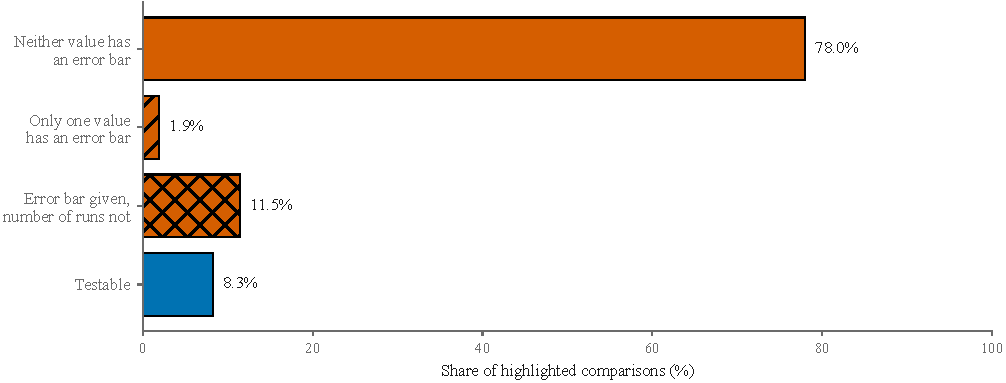
\includegraphics[width=\textwidth]{figures/untestable.pdf}
\caption{What stops a highlighted comparison from being checkable. The
overwhelming majority print no uncertainty on either side; the fully testable
slice is the small one at the bottom.}
\label{fig:untestable}
\end{figure}

\begin{table}[t]
\centering
\caption{Where tables and groups are lost between the PDF and the analysis, for
the 2025 sample. Each discard is a decision that could have gone another way, so
each is counted. The largest, by far, is tables in which no comparison group
contains exactly one bold cell---most often because nothing is bold at all.}
\label{tab:funnel}
\begin{tabular}{lr}
\toprule
Tables detected & \nTablesDetected{} \\
\quad no comparison group with exactly one bold cell & \nTablesNoOrientation{} \\
\quad yielding at least one comparison & \nTablesYielding{} \\
\midrule
Candidate comparison groups & \nCandidateGroups{} \\
\quad with exactly one bold cell and a rival & \nPctGroupsUsable{} \\
\quad of those, bold cell not extremal (discarded) & \nPctBoldNotExtremal{} \\
\midrule
Highlighted comparisons analysed & \nComparisonsTwentyFive{} \\
\bottomrule
\end{tabular}
\end{table}

Table~\ref{tab:funnel} gives the funnel from PDF to analysed comparison. The
population we measure is therefore not all results tables but the tables that
mark a winner, and within those the groups where the mark is a claim of victory
rather than a label on the authors' own row. That is the right population for
the question---a table claiming nothing cannot be checked against a claim---but
it is a filtered one, and the filter could correlate with the outcome. A cell
carrying a dispersion is harder to parse than a bare number, so tables that
report uncertainty might plausibly be the ones lost.

They are not, and the bias runs the other way. Tables that survive the filter
carry an error bar \nPctErrorBarRetained{} of the time; the tables discarded by
it, \nPctErrorBarDiscarded{}. Whatever the filter selects for, it is not the
absence of uncertainty, and the headline computed on the retained tables is if
anything the more generous of the two figures.

We also looked at \nRejectedJudged{} rejected tables to see why they were
rejected, since detecting bold in a PDF is fragile and a silent failure would
be invisible. \nRejectedNotResults{} were not results tables at all---prompt
templates, hyperparameter grids, dataset descriptions---and
\nRejectedUnmarked{} marked no winner. In \nRejectedStructural{} the bold count
matched what a reader sees but was not one cell per group. That leaves two cases
that bound the risk: one table marks its winners with background shading instead
of bold, and one may be a genuine detection failure. On twelve tables the
interval on that failure rate is \nRejectedFailCi{}, which is wide, and we
report it rather than the assertion it replaces.

Figure~\ref{fig:untestable} gives the decomposition. Of
\nComparisonsTwentyFive{} highlighted comparisons in 2025, \nPctNeitherSide{}
have no error bar on either value, \nPctOneSideOnly{} have one on only one side,
and \nPctNoNStated{} carry error bars whose number of runs is never stated. That
leaves \nPctTestable{}.

The 2024 sample gives \nPctNeitherSideTwentyFour{} and
\nPctTestableTwentyFour{}: the central figure agrees to within a point across
two samples a year apart, inside either bootstrap interval.

At the level of whole papers, \nPctWithErrorBar{} print an explicit error bar in
any results table and \nPctStatingN{} state a number of runs anywhere. Among
testable comparisons the stated run count has median \nMedianRunsTestable{},
quartiles \nRunsQOne{} and \nRunsQThree{}, and \nPctRunsLeThree{} rest on three
runs or fewer. That is small enough that the distinction between a standard
deviation and a standard error changes conclusions, and most papers that print
an error bar never say which they mean; we report results under both readings.

\section{What survives}
\label{sec:survival}

\begin{figure}[t]
\centering
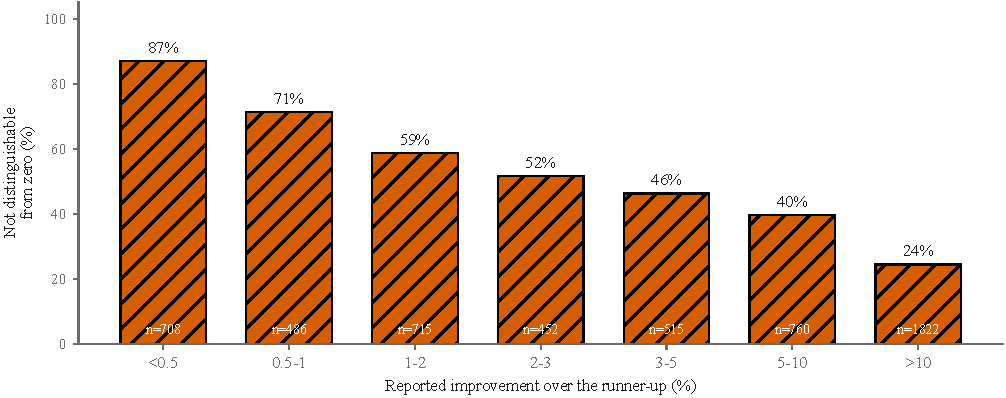
\includegraphics[width=\textwidth]{figures/gap_survival.pdf}
\caption{Within each band of reported improvement, the share that cannot be
distinguished from zero using the authors' own error bars. Failures are not
spread evenly across the range; they are concentrated in the small margins,
which is where leaderboard positions are decided.}
\label{fig:gapsurvival}
\end{figure}

Of the \nNTestable{} testable comparisons in 2025, \nCiFail{} are not
distinguishable from zero at the $5\%$ level using the numbers the authors
printed. Applying Holm--Bonferroni within each table raises this to
\nCiFailHolm{}. The correction's effect is a paired quantity---Holm can only
move a comparison from significant to not, never back---so it is estimated far
more precisely than either level: \nCiHolmDelta{} of testable comparisons change
verdict, an interval nowhere near zero.

Welch's $t$, which corrects the critical value for the stated run count, is
defined for the \nWelchDefined{} comparisons whose bars are deviations; on those
it fails \nFailWelchSubset{} against \nFailZSameSubset{} for $z$, and carrying
it through the full set gives \nFailWelchT{}
(Section~\ref{sec:sensitivity}). We keep $z$ as the headline because it is the
reading more favourable to the field, and note that a standard deviation
estimated from three runs has a relative error near one half, a second-order
uncertainty we do not propagate.

All intervals here resample papers rather than comparisons. That matters: with
an intraclass correlation of \nIcc{} and \nMeanCluster{} comparisons per paper,
the design effect is \nDesignEffect{}, so treating comparisons as independent
would report intervals about twice too narrow. A paper that asked the field to
print dispersions and then printed point estimates of its own would deserve the
objection it invited.

Figure~\ref{fig:gapsurvival} shows where the failures sit, and the pattern is
monotone: \nFailUnderHalf{} of comparisons reporting an improvement below half a
point cannot be distinguished from zero, against \nFailOverTen{} of those
reporting more than ten. Improvements that fail have a median relative size of
\nGapFailing{} against \nGapPassing{} for those that survive, and the 2024
sample agrees at \nGapFailingTwentyFour{} against \nGapPassingTwentyFour{}.
Large improvements are rarely in doubt. The margins that decide the order of a
leaderboard are the ones that cannot be supported.

\section{Could a design of that size have detected it?}
\label{sec:power}

That failing comparisons have smaller margins than surviving ones is close to
tautological: a smaller difference is harder to detect. The question worth
asking is prospective. Before the result is in, a design with $n$ runs and a
given noise level can detect differences down to some size and no smaller. The
noise level must not come from the paper being judged: a minimum detectable
effect computed from the paper's own error bar is the $z$ statistic rescaled,
and reading it as a separate finding is the observed-power fallacy
\citep{hoenig2001abuse}. We therefore take the run count from the paper and the
noise from everyone else---the median standard deviation printed by other
papers on the same benchmark and scale, or across the corpus where the benchmark
is unnamed---and compute the gap a design of that size could have detected at
\nPowerLevel{} power. That quantity does not depend on the gap the paper found
or on any dispersion it printed.

It can therefore be asked of every comparison with a stated run count, error
bars or not: \nDesignMdeN{} comparisons from \nDesignMdePapers{} papers. With a
median of \nDesignMedianRuns{} runs and a typical deviation of
\nDesignMedianSd{} points, the median detectable gap is \nDesignMedianMde{}
points, and \nPctBelowDesignMde{} of reported gaps fall below it. The share is
\nPctBelowDesignMdeTestable{} on the comparisons that print error bars and
\nPctBelowDesignMdeNoBars{} on the \nDesignMdeNoBarsN{} that print none, which
is the first statement this paper can make about that larger population. On
the testable subset the paper's own dispersion gives \nPctBelowOwnMde{}, close
enough to confirm that the borrowed noise level is not distorting the result.
The experiments are small, and the claims are made anyway.

\section{How large a test set would these gaps need?}
\label{sec:binomial}

Everything so far assumes the uncertainty that matters is variance across
training runs, which is why a comparison needs an error bar and a run count to
be testable. That is one model. For an accuracy on a fixed test set the dominant
uncertainty is over examples instead, and a binomial interval follows from the
accuracy and the number of test items alone---no error bar required. The missing
quantity is then the test-set size, not the dispersion.

This lets us ask the question in a form that needs nothing the papers did not
print. Given the gaps they report, how large would a shared test set have to be
for those gaps to be distinguishable from zero? Restricting to comparisons whose
two values both lie in $[40, 100]$ gives \nBinomComparisons{} comparisons from
\nBinomPapers{} papers---four times the base of the variance-based analysis,
because it needs no error bars. F1, BLEU and mean IoU live in that range too and
are not proportions over items, so we also report the stricter subset whose
caption or column header names an accuracy-like metric: \nBinomNamedComparisons{}
comparisons from \nBinomNamedPapers{} papers.

The median reported gap is \nBinomMedianGap{} points, and detecting it at
\nPowerLevel{} power would require about \nBinomMedianN{} test items.
\nBinomOverGsm{} of these comparisons would need a test set larger than GSM8K,
and \nBinomOverMmlu{} one larger than MMLU. On the subset that names an
accuracy-like metric the median gap is \nBinomNamedMedianGap{} points and the
requirement \nBinomNamedMedianN{} items, with \nBinomNamedOverGsm{} needing
more than GSM8K: the filter changes the population and not the answer. We
treat the two values as independent binomials, which is conservative: systems
scored on the same items are positively correlated, so a paired test needs
fewer items and the true requirement is at most what we state.

Widening the range filter to all values in $(0, 100]$ raises the median
requirement to \nBinomMedianNWide{} items, because it admits smaller gaps; the
share needing more than GSM8K moves by a point.

This analysis answers a different question from Section~\ref{sec:survival},
and the two should not be read as one. Seed variance is the noise that matters
for a claim about a training procedure on a fixed benchmark; item variance is
the noise that matters for a claim that a system is better at the task the
benchmark samples. Most papers make the second claim in words and the first in
their error bars, when they print any.

\paragraph{Against the benchmark actually used.} Where a caption names exactly
one benchmark we can do better than a hypothetical test set, because the size of
that benchmark's evaluation split is public. The smallest difference it can
resolve is then a property of the benchmark, fixed, and independent of anything
the paper prints. On \nResolutionComparisons{} such comparisons from
\nResolutionPapers{} papers, the median reported gap is \nResolutionMedianGap{}
points against a median resolution of \nResolutionMedianRes{}, and
\nResolutionPctBelow{} of the gaps fall below what the benchmark can resolve.
Treating the two systems as independent makes that resolution coarser than it
really is, so the figure is an upper bound; under paired scoring at the most
generous correlation we consider it is \nResolutionPctBelowRhoNine{}, and the
truth lies between.

% Generated by study/make_numbers.py -- do not edit by hand.
\begin{table}[t]
\centering
\caption{Reported gaps against the resolution of the benchmark they are measured on. The pattern is the check on the method: the largest evaluation split has the smallest share of unresolvable gaps, and the smallest splits have nearly all of them.}
\label{tab:resolution}
\begin{tabular}{lrrr}
\toprule
Benchmark & Split size & Comparisons & Gap below resolution \\
\midrule
ImageNet & 50{,}000 & 610 & 34.3\% \\
CIFAR-10 & 10{,}000 & 497 & 49.7\% \\
CIFAR-100 & 10{,}000 & 283 & 55.5\% \\
MMLU & 14{,}042 & 58 & 43.1\% \\
GSM8K & 1{,}319 & 79 & 79.7\% \\
SST-2 & 872 & 38 & 50.0\% \\
WinoGrande & 1{,}267 & 79 & 98.7\% \\
TruthfulQA & 817 & 43 & 79.1\% \\
\bottomrule
\end{tabular}
\end{table}


Table~\ref{tab:resolution} gives the breakdown, and the pattern in it is the
internal check on the method: ImageNet, with the largest evaluation split, has
the smallest share of unresolvable gaps, while WinoGrande and TruthfulQA, with
around a thousand items each, have almost nothing else. A benchmark of a
thousand items cannot resolve a one-point difference, and one-point differences
are what the field reports on it.

\section{How much is a definitional choice?}
\label{sec:sensitivity}

Several decisions in the pipeline are not forced by the data, and they matter
more than sampling does. Table~\ref{tab:span} gives the failure rate under each,
with the population each row is computed on. Over the rows that share the full
population of \nSpanN{} testable comparisons the span is \nSpanLow{} to
\nSpanHigh{}, against a bootstrap interval of \nCiFail{} that captures sampling
alone---definitional uncertainty is more than twice the statistical kind.

The headline sits at a definite place in that span, and we say where. It reads
unlabelled bars as standard deviations, takes the two values as independent,
and uses $z$ rather than $t$; the first and third favour the field, the second
does not. The check on it is the subset where authors state what their error
bar means, which fails at \nLabelledOnlyFail{}. The width of the span is not a
weakness to be argued away---it exists because the papers do not print which
convention they used, which is the paper's own thesis applied to itself.

\begin{table}[t]
\centering
\caption{Both headline figures under each decision the pipeline had to make,
each row on a stated population. The span across conventions is far wider than
the sampling interval in both cases, because the source papers do not state
which convention they used, and wider still for checkability than for the
failure rate.}
\label{tab:span}
\begin{tabular}{lrr}
\toprule
& $n$ & Not distinguishable from zero \\
\midrule
As reported: two-sided $z$, Holm within table & \nSpanN{} & \nPctFail{} \\
Welch's $t$ where a run count defines it & \nSpanN{} & \nFailWelchT{} \\
One-sided $z$ & \nSpanN{} & \nFailOneSided{} \\
Unlabelled bars read as standard errors & \nSpanN{} & \nUnlabelledAsSemFull{} \\
Compared values correlated at $\rho = \nRhoHalf{}$ & \nSpanN{} & \nFailRhoHalf{} \\
Compared values correlated at $\rho = \nRhoNine{}$ & \nSpanN{} & \nFailRhoNine{} \\
Only bars whose meaning is stated & \nLabelledOnlyN{} & \nLabelledOnlyFail{} \\
Run count taken from the caption only & \nStrictN{} & \nStrictFail{} \\
Tie-marked comparisons removed & & \nFailExcludingTie{} \\
Holm family the paper, not the table & \nSpanN{} & \nFailHolmPaper{} \\
\midrule
Sampling interval, conventions held fixed & \nSpanN{} & \nCiFail{} \\
\midrule
\multicolumn{3}{l}{\emph{And the share that is checkable at all}} \\
As reported & \nComparisonsTwentyFive{} & \nPctTestable{} \\
Run count taken from the caption only & \nComparisonsTwentyFive{} & \nStrictTestable{} \\
Every unlabelled bar read as a standard error & \nComparisonsTwentyFive{} & \nTestableAsSem{} \\
\bottomrule
\end{tabular}
\end{table}

\paragraph{Where a run count may come from.} A table's caption sometimes states
how many runs produced its means; more often the count appears once in the
experimental setup and is meant to govern everything. Counting only captions
gives \nStrictTestable{} testable and \nStrictFail{} failing; allowing a count
stated anywhere in the paper to govern its tables gives \nPctTestable{} and
\nPctFail{}. We report the second throughout. The choice matters because the two
sets of papers barely overlap: of the papers that print an explicit error bar,
only \nPctErrorBarPapersStatingRuns{} state a number of runs anywhere
(\nPapersErrorBarAndRuns{} papers print both, \nPapersErrorBarOnly{} print an
error bar and no count). Reporting a dispersion without saying what it is a
dispersion over is itself the most common failure mode we see.

\paragraph{Whether the two values are independent.} Our test treats the winner
and the runner-up as independent samples. They are not: in almost every table
under study the two methods are evaluated on the same fixed test set, so their
errors are positively correlated and the difference is a paired quantity, with
$\mathrm{Var}(A - B) = \sigma_A^2 + \sigma_B^2 - 2\rho\sigma_A\sigma_B$.
Assuming $\rho = 0$ inflates the standard error of the difference, which makes a
gap harder to call significant and therefore makes \emph{our own} failure rate
too high. Papers do not print the covariance, so we report the range: at
$\rho = 0.5$ the failure rate is \nFailRhoHalf{} rather than \nPctFail{}, and
even at $\rho = \nRhoNine{}$ it is \nFailRhoNine{}. We quote the independent figure in
the abstract because it is the assumption the source papers' own reporting
supports, and we flag here that it is the end of the range least favourable to
the field. The finding does not depend on the choice: under every assumption we
can defend, at least a fifth of checkable improvements are indistinguishable
from zero.

\paragraph{Checkability moves further than survival does.} The share that can be
checked at all is the more convention-dependent of our two headline figures, and
we owe the reader that plainly. A standard error is
already the dispersion of a mean, so a comparison whose bars are standard errors
needs no run count: reading every unlabelled bar that way makes
\nTestableAsSem{} of comparisons testable rather than \nPctTestable{}, while
demanding the run count come from the caption leaves \nStrictTestable{}. That is
a factor of \nTestableSpanFactor{} between the ends, against a sampling interval
of about two points. We report \nPctTestable{} because it follows from the
conventions we can defend, and the claim in our title survives the whole range:
even at the most generous end, four highlighted comparisons in five cannot be
checked.

\paragraph{What an unlabelled error bar means.} A paper that prints
$82.4 \pm 0.3$ usually does not say whether $0.3$ is a standard deviation or a
standard error, and the two differ by $\sqrt{n}$. On the \nNUnlabelled{}
unlabelled comparisons that carry a run count, reading every bar as a standard
deviation gives \nUnlabelledAsStd{} failing and as a standard error
\nUnlabelledAsSem{}; carried into the full population, with labelled bars read
as labelled, the second gives \nUnlabelledAsSemFull{}. We use the first, the
more conservative. The subset where authors do say which they mean fails at
\nLabelledOnlyFail{}, close to the \nPctFail{} headline, which is the evidence
that the convention we assume is not distorting the result.

\section{Threats to validity}
\label{sec:threats}

\paragraph{The extractor could be wrong.} This is the threat that matters, and
we attack it three ways, of which the third is the one that scales. First, we rendered sampled tables as images and compared
them against the extracted values by eye. This found five distinct bugs, each of
which had produced a confident and wrong version of these numbers: error bars
set as subscripts being paired with the neighbouring column's mean; a page
number extracted as a runner-up; the neighbouring column of a two-column layout
being swept in; a table's orientation misread; and a run count taken from a row
label reading ``top 100''. We report them because the reader has no other way to
calibrate what remains. Second, we built a second extractor on entirely
different principles---grid detection rather than span geometry---and measured
agreement: it confirms \nCrosscheckConfirmation{} of \nCrosscheckValues{} values
carrying an error bar. Inspection of the disagreements shows most are failures
of the second extractor, so this is a lower bound rather than a central
estimate. Third, and most usefully, every NeurIPS paper since 2021 answers a
mandatory checklist question that is nearly the one we ask: \emph{does the paper
report error bars suitably and correctly defined?} Only \nCheckNoButHasBar{}
papers answering \emph{no} turn out to have a table error bar, so the extractor
agrees with author self-report on \nCheckPrecision{} cases---hundreds of papers
rather than the handful a person can inspect.

Neither precision check bounds the quantity the headline depends on, which is
recall: an error bar present in the PDF and missed falls silently into ``neither
value has an error bar'', and every one of our six bugs could only have moved
the headline in the same direction. We therefore sampled tables the extractor
had called empty and looked at them. An audit of eighteen found one miss---the
sixth bug, values written $76.63(\pm 3.98)$ with the bracket wrapping the
symbol---and correcting it across the corpus moved the headline by
\nHeadlineMoveSixth{}, not the eight points that extrapolating from that audit
would have predicted. We then audited \nRecallThreeJudged{} more tables on the
corrected extractor and found \nRecallThreeMissed{} misses
(\nRecallThreeCi{}). The audit also turned up three conventions worth naming
rather than counting as failures: a caption that bounds the standard error
instead of printing it per cell, one that marks significant differences with a
dagger from a permutation test, and one that bolds every result tied for best.
In each the extractor is right that no error bar is present, and in each a
reader is nonetheless given something to check against.

That interval is the dominant uncertainty in this paper, and it is wider than
the sampling interval. Propagating it, the share of comparisons carrying no
error bar is \nHeadlineWithExtraction{} rather than the
\nCiNeitherSide{} that sampling alone would suggest. We quote both, because a
paper arguing that published intervals omit their largest source of uncertainty
has no business omitting its own.

\paragraph{The testable subset is small and may be unrepresentative.} The
\nNTestable{} testable comparisons come from \nPapersContributing{} distinct
papers. Papers that report uncertainty are plainly not a random sample of
papers; if anything they are the more careful ones, which would make the failure
rate among them a \emph{lower} bound on the rate that would be found if every
paper reported enough to check. We cannot verify that, and say so.

\paragraph{Bold is a proxy for a claim, and an imperfect one.} Some papers bold
nothing, some bold an entire row, and some use bold for emphasis unrelated to
ranking. Two discards follow, and both are large enough to state rather than
describe. Groups without exactly one bold cell and a rival are dropped. Of the
groups that remain, \nPctBoldNotExtremal{} have a bold cell that is not the best
value in its group---authors marking their own method regardless of whether it
won---and those are dropped too, since no victory is being claimed. What we
analyse is therefore the set of claimed wins, not of all highlighted cells, and
the funnel in Section~\ref{sec:checkable} gives every count.

\paragraph{Some tables mark ties, and we would score a tie as a failure.} A
paper that bolds the best result and marks everything statistically
indistinguishable from it has declared those pairs ties, and the convention does
concentrate where it hurts: it appears in \nPctTieTables{} of all tables but
\nPctTieTestable{} of the testable subset, where those comparisons fail at
\nFailAmongTieMarked{}. Removing them moves the failure rate to
\nFailExcludingTie{}. Appendix~\ref{app:ties} gives the detail.

\paragraph{Our two best pieces of evidence appear to contradict each other.} The
recall audit says the extractor misses almost nothing; the checklist says
\nCheckYesNoTable{} NeurIPS papers claim error bars we cannot find. Reading
those justifications resolves it: most do not claim an error bar in a results
table at all, the commonest at \nJustSeeds{} being that several seeds were used,
which is averaging rather than reporting dispersion. What the checklist records
is not what it asks. Appendix~\ref{app:checklist} gives the breakdown and rules
out the two extraction limits that could have produced the same gap.

\paragraph{Large PDFs are skipped.} A size cap excludes a small number of
image-heavy papers, which are not a random subset. We report the count rather
than lowering the cap for speed.

\section{Related work}
\label{sec:related}

\paragraph{How to report uncertainty.} A line of work tells authors what they
should print. \citet{dodge2019show} argue for reporting the full distribution of
results over hyperparameter search rather than a single tuned number;
\citet{bouthillier2021accounting} decompose the variance of a benchmark result
into its sources and show how many seeds are needed to detect a given effect;
\citet{miller2024adding} derives the error bars a language model evaluation
should carry, and \citet{bowyer2025position} shows that the usual normal
approximation fails on the small evaluation sets now common. These papers say
what a correct interval looks like. We measure how often any interval is
printed at all, which is prior to whether it is correct.

\paragraph{Whether reported gains are real.} A second line re-runs a
literature under a common protocol and finds the gains smaller than claimed or
absent: \citet{henderson2017deep} in deep reinforcement learning,
\citet{musgrave2020metric} in metric learning, \citet{dacrema2019really} in
neural recommendation. \citet{saidi2024unraveling} find the same pattern across
machine-learning-driven science and attribute it partly to publication bias.
Each of these requires re-running the methods, which bounds them to one subfield
at a time. Our measurement needs only the printed page, so it covers whole
venues, at the cost of saying nothing about whether any individual result is
true.

\paragraph{Hand audits of reporting practice.} A line of studies asks our
question by reading papers one at a time, and Table~\ref{tab:audits} sets them
beside this one. \citet{bergkirkpatrick2012empirical} and \citet{dror2018hitchhiker}
count significance testing in computational linguistics; \citet{gundersen2018state}
score AAAI and IJCAI papers for what a reproduction would need;
\citet{kirly2018nips} review NeurIPS 2017 and find roughly a third reporting
confidence intervals; \citet{christodoulou2024confidence} annotate 221 MICCAI
2023 papers and find more than half assessing no variability at all;
\citet{agarwal2021deep} show that point estimates over a handful of runs
misorder deep reinforcement learning methods. \citet{pineau2021improving}
describe the NeurIPS checklist we read in Section~\ref{sec:threats}. Their
figures are not ours on a larger corpus, because the definitions differ: an
error bar anywhere in a paper, a confidence interval, a significance test, and
an explicit interval in a results table are four different events, and ours is
the narrowest. Our paper-level \nPctWithErrorBar{} is accordingly below the
earlier figures, not between them.

\begin{table}[t]
\centering
\caption{Audits of reporting practice. Each earlier study labels papers by
hand, at the scale of a person; this one labels comparisons by machine, and
Section~\ref{sec:threats} measures the instrument against tables read by hand.}
\label{tab:audits}
\small
\begin{tabular}{lllll}
\toprule
Study & Venue & Labelled by & Unit & Headline \
\midrule
\citet{bergkirkpatrick2012empirical} & ACL & hand & paper & significance tests rarely reported \
\citet{dror2018hitchhiker} & ACL, TACL 2017 & hand & paper & about a third test significance \
\citet{gundersen2018state} & AAAI, IJCAI & hand & paper & most omit what a reproduction needs \
\citet{kirly2018nips} & NeurIPS 2017 & hand & paper & about a third report intervals \
\citet{christodoulou2024confidence} & MICCAI 2023 & hand & paper & over half assess no variability \
This paper & NeurIPS, ICML 2024--25 & machine & comparison & \nPctNeitherSide{} print no error bar \
\end{tabular}
\end{table}

Their limit is the one manual annotation always has, and it is the gap this work
fills. A person can read a few hundred papers, and can record only what happens
at the level of a paper: whether it reports variability somewhere. But the unit
a results table claims in is not the paper, it is the individual comparison, and
a paper printing one error bar in an appendix while its main table prints none
counts as reporting variability under a paper-level audit and as unchecked under
ours. Working at the comparison is what makes \nComparisonsTwentyFive{}
observations available where hand annotation yields a few hundred, and it is
what makes the questions in Sections~\ref{sec:survival} to \ref{sec:binomial}
askable at all: whether the specific difference being claimed survives its own
error bars, whether a design of that size could have detected it, and whether
the benchmark it was measured on can resolve it. None of the three is answerable
from a paper-level label. What automation costs is the judgement a human brings
to an ambiguous table, which is why Section~\ref{sec:threats} spends its length
measuring what ours gets wrong.

\paragraph{Statistical practice as an object of study.} A second group asks the
question of one subfield each. \citet{card2020with} compute the statistical
power of natural language processing experiments and find most underpowered for
the effects they report, and \citet{colas2018how} do the same for deep
reinforcement learning; the comparison of a claimed gap against what a
benchmark can resolve (Section~\ref{sec:binomial}) is theirs, carried out here
by machine on every named-benchmark comparison in two venues rather than by
hand on a few tasks. \citet{reimers2017reporting} show that a single run can
misorder methods that several runs order correctly, and \citet{ulmer2022experimental}
turn such findings into a standard; we measure how far the standard is from
practice. The nearest ancestor in method is outside machine learning:
\citet{nuijten2016prevalence} recompute the $p$-values printed in a quarter of
a million psychology papers from the test statistics beside them, which is a
corpus-scale re-test of published claims from the printed page alone.
\citet{marie2021scientific} hand-annotate machine translation papers for
evaluation practice and find the field's conventions drifting; they establish
what careful manual annotation can see, at the scale manual annotation permits.
\citet{tang2020showing} show that the reporting practice proposed by
\citet{dodge2019show} can itself mislead as usually implemented. We differ from
all three in unit and scale: every highlighted comparison in \nPapersTotal{}
papers, at the cost of reading only what is printed.

\paragraph{Extracting results from papers.} \citet{hou2019identification} and
\citet{kardas2020axcell} extract result tables from machine learning PDFs to
populate leaderboards: the same mechanics, the opposite purpose, since
leaderboard extraction wants the winning number and can ignore a missing error
bar. We know of no released annotation of error-bar presence against which an
extractor could be scored, so Section~\ref{sec:threats} builds one.

\section{Discussion}
\label{sec:discussion}

The cheapest fix is not more statistics. It is printing three quantities that
authors already have: a dispersion on each value in the main comparison, and the
number of runs behind them. A paper that prints those becomes checkable by
anyone, forever, at no cost to the authors.

A second fix costs nothing at all, because it applies before the experiment
rather than after. The smallest difference a benchmark can resolve follows from
its evaluation split and belongs to the benchmark, not to any paper.
Appendix~\ref{app:mde} tabulates it, and some values are startling: AIME's
\nAimeItems{} items cannot distinguish anything below about \nAimeMde{} points,
HumanEval's \nHumanevalItems{} below \nHumanevalMde{}. An author who consults it
first will sometimes find the sentence cannot be written, which is the point.

The descriptive result is what it is; the prescriptive one follows from it
immediately, and is small.

% The mandatory statements below do not count toward the nine-page limit,
% so the main text ends here.
\label{lastmainpage}

\subsubsection*{Reproducibility statement}
The corpus is defined by a venue, a year, and a random seed, and is rebuilt by
one command from the open proceedings. Every number in this paper is a macro
generated from a recorded run; a number typed into the LaTeX by hand fails the
build. The extraction pipeline, the analysis, the per-comparison database and
the validation renderings are released.

\subsubsection*{AI use statement}
The authors used a large language model as a coding assistant throughout: to
write and revise the extraction and analysis code, to draft and edit prose, and
to search the literature. Every empirical number in the paper was produced by
the released code and checked against its run record. All six extractor bugs
described in Section~\ref{sec:threats} were found by the authors inspecting
rendered tables against extracted values---five in the first pass and the sixth
in the recall audit; that inspection, and every methodological decision, was
made by the authors, who take full responsibility for the paper's claims.

\subsubsection*{Ethics statement}
This work audits published papers in aggregate. We report no individual paper as
an example of a failure, name no authors, and release the per-comparison
database with paper identifiers so that our claims can be checked, not so that
particular papers can be criticised. The pattern is a property of the field's
conventions, not of the people following them.


\bibliographystyle{iclr2027_conference}
\bibliography{refs}

\appendix

\section{Tie marking}
\label{app:ties}

A paper that bolds the best result and marks every result not statistically
distinguishable from it has already declared those pairs to be ties; counting
them as failed comparisons would inflate our failure rate. The convention is
real, and it concentrates exactly where it does the most damage. Captions
claiming statistical indistinguishability appear in \nPctTieTables{} of all
tables but \nPctTieTestable{} of the testable subset---a tenfold
enrichment---because the papers careful enough to print dispersions are the ones
most likely to mark ties. Those comparisons fail at \nFailAmongTieMarked{}
against \nPctFail{} overall, which is what one would expect of pairs the authors
had already declared indistinguishable.

The mechanism is therefore confirmed and the magnitude is small. Removing
tie-marked comparisons moves the failure rate from \nPctFail{} to
\nFailExcludingTie{}, because the convention remains rare even after the
enrichment. The commoner convention, marking the second-best result
(\nPctSecondBest{} of tables), is not a tie claim and is left in.

\section{What each benchmark can resolve}
\label{app:mde}

Table~\ref{tab:mde} gives, for each benchmark in common use, the smallest
difference in accuracy it can distinguish from zero at $\alpha = 0.05$ and
\nPowerLevel{} power. The quantity depends only on the published evaluation
split, so it is fixed, checkable, and available before an experiment is run.

Two readings are shown. The independent-binomial column treats the two systems
as unrelated, which is conservative; the paired column assumes they are scored
on the same items with a correlation of \nPairedRho{}, which is closer to how
benchmarks are actually used and resolves finer. Values are given at three
accuracies because a binomial variance is largest near one half, so a benchmark
resolves more finely at the top of its scale than in the middle.

% Generated by study/make_numbers.py -- do not edit by hand.
\begin{table}[t]
\centering
\small
\caption{Smallest difference in accuracy, in percentage points, that each benchmark can distinguish from zero at 80 per cent power. Columns give the independent reading at three accuracies and the paired reading at 70 per cent. A property of the benchmark, not of any paper.}
\label{tab:mde}
\begin{tabular}{lrrrrr}
\toprule
Benchmark & Split & At 50\% & At 70\% & At 90\% & Paired, 70\% \\
\midrule
AIME & 30 & 36.17 & 33.15 & 21.70 & 23.44 \\
HumanEval & 164 & 15.47 & 14.18 & 9.28 & 10.03 \\
GPQA Diamond & 198 & 14.08 & 12.90 & 8.45 & 9.12 \\
MBPP & 500 & 8.86 & 8.12 & 5.32 & 5.74 \\
OpenBookQA & 500 & 8.86 & 8.12 & 5.32 & 5.74 \\
MATH-500 & 500 & 8.86 & 8.12 & 5.32 & 5.74 \\
SWE-bench Verified & 500 & 8.86 & 8.12 & 5.32 & 5.74 \\
TruthfulQA & 817 & 6.93 & 6.35 & 4.16 & 4.49 \\
SST-2 & 872 & 6.71 & 6.15 & 4.03 & 4.35 \\
ARC-Challenge & 1{,}172 & 5.79 & 5.30 & 3.47 & 3.75 \\
WinoGrande & 1{,}267 & 5.57 & 5.10 & 3.34 & 3.61 \\
GSM8K & 1{,}319 & 5.45 & 5.00 & 3.27 & 3.54 \\
PIQA & 1{,}838 & 4.62 & 4.24 & 2.77 & 2.99 \\
ARC-Easy & 2{,}376 & 4.06 & 3.72 & 2.44 & 2.63 \\
BoolQ & 3{,}270 & 3.46 & 3.18 & 2.08 & 2.25 \\
MATH & 5{,}000 & 2.80 & 2.57 & 1.68 & 1.82 \\
QNLI & 5{,}463 & 2.68 & 2.46 & 1.61 & 1.74 \\
CoQA & 7{,}983 & 2.22 & 2.03 & 1.33 & 1.44 \\
DROP & 9{,}536 & 2.03 & 1.86 & 1.22 & 1.31 \\
MNLI & 9{,}815 & 2.00 & 1.83 & 1.20 & 1.30 \\
CIFAR-10 & 10{,}000 & 1.98 & 1.82 & 1.19 & 1.28 \\
CIFAR-100 & 10{,}000 & 1.98 & 1.82 & 1.19 & 1.28 \\
HellaSwag & 10{,}042 & 1.98 & 1.81 & 1.19 & 1.28 \\
SQuAD & 10{,}570 & 1.93 & 1.77 & 1.16 & 1.25 \\
MMLU-Pro & 12{,}032 & 1.81 & 1.66 & 1.08 & 1.17 \\
MMLU & 14{,}042 & 1.67 & 1.53 & 1.00 & 1.08 \\
ImageNet & 50{,}000 & 0.89 & 0.81 & 0.53 & 0.57 \\
\bottomrule
\end{tabular}
\end{table}


\section{The checklist and the recall audit}
\label{app:checklist}

The recall audit says the extractor misses almost nothing; the checklist says
\nCheckYesNoTable{} NeurIPS papers claim error bars we cannot find. Both cannot
be right unless the claim means something other than what we measure, so we read
what those justifications actually say.

They mostly do not claim an error bar in a results table. The commonest, at
\nJustSeeds{}, is that several random seeds were used---which is averaging, not
reporting dispersion. Another \nJustTest{} report having run a significance
test, \nJustFigure{} point to a figure and \nJustAppendix{} to an appendix, and
\nJustNone{} make no recognisable claim at all. The two measurements are
consistent, and the disagreement is the finding: what the checklist records is
not what it asks.

Two extraction limits could have produced the same gap and do not. Papers longer
than our \nMaxPages{}-page window are \nPctLongPapers{} of the corpus and have a
\emph{lower} error-bar rate (\nErrorBarLong{} against \nErrorBarShort{}), so
truncation is not hiding a mass of error bars in appendices. And \nPctNoTable{}
of papers yield no detected table at all; excluding them raises the paper-level
rate from \nPctWithErrorBar{} to \nPctWithErrorBarConditional{}, and we report
both. The paper-level statistic reads every detected table, not only those
reaching the comparison stage: of the \nPapersTablesNoComparison{} papers whose
tables yield no comparison, \nPapersTablesNoComparisonWithBar{} are correctly
credited with an error bar. Only papers with no detected table are scored blind.

\end{document}
